\chapter[Conocimientos previos]{Conocimientos previos sobre las tecnologías usadas.}

En este segundo capítulo vamos a explicar cuales son y los conocimientos previos que teníamos sobre las tecnologías que hemos usado en el proyecto, así como una breve explicación de su funcionamiento, para que se usa y explicación breve sobre su historia y sus recientes versiones.

El elemento principal usado en el proyecto es el lenguaje de programación Java, en cual se programa tanto la aplicación web como la aplicación en el móvil, pero además de los diferentes SDK de Android y de Google App Engine, hace falta muchas otras tecnologías y lenguajes como pueden ser SQL, XML, UML, GIT. Además de los conocimientos básicos sobre criptografía de clave pública necesarios para realizar todo el proceso de firma digital.   

\section{El lenguaje de programación Java}

Java es un lenguaje de programación orientado a objetos que fue diseñado por Jame Gosling\footnote{Para más información sobre Jame Gosling: \url{http://en.wikipedia.org/wiki/James\_Gosling}} para Sun Microsystems, que recientemente ha sido comprada por Oracle Corporation. Fue lanzado en 1995 y fue el centro de toda la plataforma Java de Sun Microsystems. Es un lenguaje con una sintaxis muy parecida a C o C++, pero con la gran ventaja de que el manejo de punteros y objetos es automático, al igual que la recogida de basura.

Java es un lenguaje en el que hay que compilar los código fuentes para crear unos archivos intermedios llamados bytecodes, los archivos *.class, que luego serán interpretados por la máquina virtual de Java (JVM), que depende de la arquitectura en la que se quiera ejecutar la aplicación java. Gracias a esto se puede decir que java es un lenguaje multiplataforma, lo que significa que un mismo código java se puede ejecutar en un linux, en un windows, un mac o cualquier otro sistema para el cual exista una máquina virtual, lo que en inglés se llama "write once, run anywhere" (WORA). Además de esta gran ventaja Java es un lenguaje de propósito general, concurrente, basado en clases y orientado a objetos. Java es el segundo lenguaje de programación más popular de 2012, gracias a las aplicaciones web cliente-servidor que tienen tanto auge en estos momentos, como podemos ver en la figura \ref{fig:indicetiobe}.

\begin{figure}
  \centering
    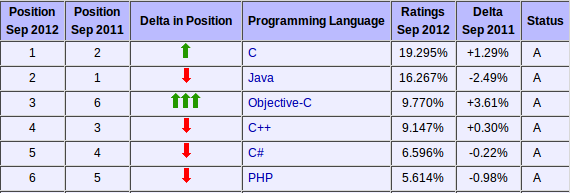
\includegraphics[scale=0.9]{./ConocimientosPrevios/imagenes/indiceTiobe.png}
  \caption{Índice tiobe en septiembre del 2012. \url{http://www.tiobe.com/}}
  \label{fig:indicetiobe}
\end{figure} 

%TODO: revisar este párrafo, por si hay que ponerlo mejor en la historia
La implementación original y las referencias del compilador de java, máquinas virtuales y las librerías de clases fue desarrollado por Sun en 1995, pero en el 2007 gracias a la lavor de la comunidad, Sun Microsystem cambio la licencia de todas las tecnologías Java a GNU General Public License, por lo que se abría la posibilidad a que se crearan versiones alternativas de compiladores bajo licencia GNU como GNU Compiler para Java o GNU Classpath.

En el proyecto la versión usada fue la versión Java SE 6.

\subsection{Historia}

Originalmente Java nació como un proyecto de James Gosling, Mike Sheridan, and Patrick Naughton en 1991, y estaba diseñado para una televisión interactiva pero era muy avanzado para lo que la industria de la televisión por clave de la época podía necesitar. En su origen fue llamado como Oak, por problemas con el nombre, ya que era una marca registrada cambiaron a llamarlo Green y posteriormente ya lo renombraron a Java como en la actualidad. Hay muchas teorías sobre el porque se llama Java, una de ellas es que había una cafetería llamada Java Coffe donde Jame, Mike and Patrick pasaron muchas horas consumiendo café.

La idea de James Gosling era crear una máquina virtual y un lenguaje de programación con la sintaxis y la estructura de C/C++ para que la curva de aprendizaje fuera muy suave para programadores que en la época sabían C/C++.

Sun Microsystem lanzó Java 1.0 en 1995, con la principal característica de que una vez escrito un código fuente no había que modificarlo para que funcionara en las diferentes máquinas, lo que anteriormente hemos llamado con el acrónimos en inglés WORA (Write Once, Run Anywhere). Rápidamente todos los navegadores de la época empezaron a soportar applet java en las páginas web, por lo que Java se volvió muy popular en la época. La nueva versión Java 2 fue lanzada en 1998-1999 y con ella llegarón las distinciones para las diferentes plataformas, como por ejemplo Java2EE para aplicaciones corporativas o una versión ligera llamada Java2ME que estaba diseñada para funcionar en los diferentes telefónos de la época, y todas las demás que se agrupan en la versión Java2SE, que es la versión estandar.

En 1997, Sun Microsystem intentó formalizar Java mediante una norma ISO/IEC pero se retiró del proceso y dio todo el control a la comunidad. Sun ofrecia implementaciones gratuitas y generaba dinero vendiendo algunas licencias de productos como Java Enterprise System. Una cosa importante es que Sun distingue entre el SDK (Kit de desarrollo) y el JRE (Entorno de ejecución) en el que van incluidos los compiladores, debugger, etc.

El 13 de noviembre del 2006, Sun lanzó Java gratis y software libre, bajo la licencia GNU General Public License (GPL). El proceso concluyó el 8 de mayo del 2007.

En 2009-2010 Oracle Corporation compró Sun Microsystem por lo que Java actualmente pertenece a Oracle.

\subsection{Versiones}

\begin{itemize}

	\item \textbf{JDK 1.0}  (23 de enero de 1996): Primer lanzamiento
	
	\item \textbf{JDK 1.1} (19 de febrero de 1997): Las primeras características añadidas fuero una reestructuración intensiva del modelo de eventos AWT (Abstract Windowing Toolkit), clases internas (inner classes), JavaBeans, JDBC (Java Database Connectivity), para la integración de bases de datos y RMI (Remote Method Invocation).
	
     (8 de diciembre de 1998): Recibió el nombre en clave Playground. Esta y las siguientes versiones fueron recogidas bajo la denominación Java 2 y el nombre "J2SE" (Java 2 Platform, Standard Edition), reemplazó a JDK para distinguir la plataforma base de J2EE (Java 2 Platform, Enterprise Edition) y J2ME (Java 2 Platform, Micro Edition). 
    Se añadieron las siguientes mejoras, la palabra reservada strictfp, reflexión en la programación, la API gráfica ( Swing) fue integrada en las clases básicas, la máquina virtual (JVM) de Sun fue equipada con un compilador JIT (Just in Time) por primera vez, Java Plug-in, Java IDL, una implementación de IDL (Lenguaje de Descripción de Interfaz) para la interoperabilidad con CORBA y Colecciones.

    \item \textbf{J2SE 1.3} (8 de mayo de 2000): Recibió el nombre en clave Kestrel. Los cambios más notables fueron: la inclusión de la máquina virtual de HotSpot JVM, RMI fue cambiado para que se basara en CORBA, JavaSound, se incluyó el Java Naming and Directory Interface (JNDI) en el paquete de bibliotecas principales (anteriormente disponible como una extensión), Java Platform Debugger Architecture (JPDA).

    \item \textbf{J2SE 1.4} (6 de febrero de 2002): Recibió el nombre en clave Merlin. Este fue el primer lanzamiento de la plataforma Java desarrollado bajo el Proceso de la Comunidad Java como JSR 59. Las principales características que se le añadieron fueron palabra reservada assert, expresiones regulares modeladas al estilo de las expresiones regulares Perl, encadenación de excepciones, non-blocking NIO (New Input/Output), logging API, API I/O para la lectura y escritura de imágenes en formatos como JPEG o PNG, parser XML integrado y procesador XSLT (JAXP), seguridad integrada y extensiones criptográficas (JCE, JSSE, JAAS), Java Web Start incluido.
    
    \item \textbf{J2SE 5.0} (30 de septiembre de 2004): Recibió el nombre en clave Tiger. Estos fueron los cambios mas importantes, plantillas (genéricos), metadatos, también llamados anotaciones, permite a estructuras del lenguaje como las clases o los métodos, ser etiquetados con datos adicionales, que puedan ser procesados posteriormente por utilidades de proceso de metadatos, autoboxing/unboxing, conversiones automáticas entre tipos primitivos (Como los int) y clases de envoltura primitivas (Como Integer), enumeraciones, varargs (número de argumentos variable), el último parámetro de un método puede ser declarado con el nombre del tipo seguido por tres puntos (por ejemplo \textit{void drawtext(String... lines)}). En la llamada al método, puede usarse cualquier número de parámetros de ese tipo, que serán almacenados en un array para pasarlos al método, bucle for mejorado, La sintaxis para el bucle for se ha extendido con una sintaxis especial para iterar sobre cada miembro de un array o sobre cualquier clase que implemente Iterable, como la clase estándar Collection, de la siguiente forma:
\begin{figure}
	\begin{lstlisting}[language=Java]
	 void displayWidgets (Iterable<Widget> widgets) {
		 for (Widget w : widgets) {
		     w.display();
		 }
	 }
	\end{lstlisting}
	\caption{Código ejemplo código for mejorado.}
\end{figure}

    \item \textbf{Java SE 6} (11 de diciembre de 2006): Recibió el nombre en clave Mustang. En esta versión, Sun cambió el nombre "J2SE" por Java SE y eliminó el ".0" del número de versión. Los cambios más importantes introducidos en esta versión fueron un nuevo marco de trabajo y APIs que hacen posible la combinación de Java con lenguajes dinámicos como PHP, Python, Ruby y JavaScript, el motor Rhino, de Mozilla, una implementación de Javascript en Java, un cliente completo de Servicios Web y soporta las últimas especificaciones para Servicios Web, mejoras en la interfaz gráfica y en el rendimiento.
    
    \item \textbf{Java SE 7}: Su nombre en clave es Dolphin. Su lanzamiento fue en julio de 2011. Y las principales nuevas características fuero: soporte para XML dentro del propio lenguaje, un nuevo concepto de superpaquete, soporte para closures, introducción de anotaciones estándar para detectar fallos en el software.

\end{itemize}

\section{El entorno de programación Eclipse.}

Eclipse es un entorno integral de desarrollo que consta de un entorno de desarrollo integrado (IDE) y es extensible mediante plugins que está escrito en Java. Puede ser usado para una larga lista de lenguajes de programación como pueden ser,  C, C++, Haskell, Perl, PHP, Python, Android y un largo etcetera. Fue originalmente desarrollado por IBM y fue lanzado con la licencia de software Eclipse Public License\footnote{Para más información visite: \url{http://en.wikipedia.org/wiki/Eclipse\_Public\_License}} la cual es una licencia de software libre. El SDK de Eclipse es libre y tiene licencia open source por lo que cualquier persona con los conocimientos puede programar el puglin que necesite para Eclipse. Fue el primer entorno de programación que funcionó bajo GNU Classpath y que funcionaba sin problemas con IcedTea. En la figura \ref{fig:pantallaEclipse} se puede ver el aspecto que tiene.

\begin{figure}
  \centering
    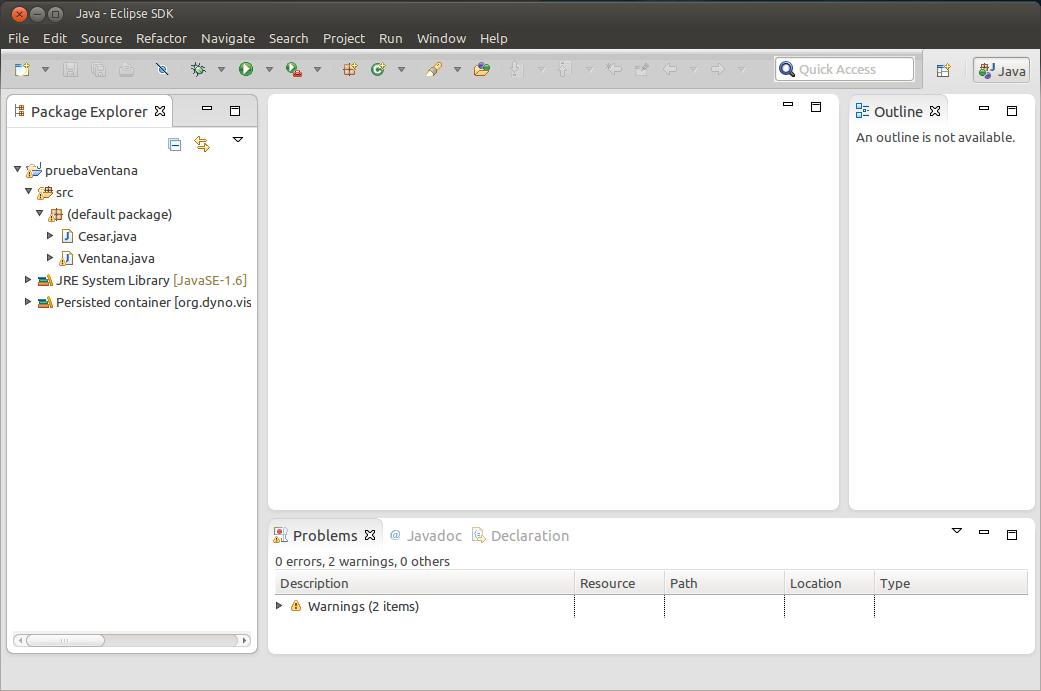
\includegraphics[scale=0.5]{./ConocimientosPrevios/imagenes/pantallaEclipse.png}
  \caption{Eclipse 4.2 Juno.}
  \label{fig:pantallaEclipse}
\end{figure} 

\subsection{Historia}

Eclipse comenzó como un proyecto de IBM Canadá. En noviembre de 2001 se creó un grupo de empresas para promover el desarrollo de Eclipse como software libre, los miembros iniciales eran Borland, IBM, Merant, QNX Software Systems, Rational Software, Red Hat, SuSE, TogetherSoft and WebGain. Finalmente en enero de 2004 se creó la Eclipse Foundation. 

%TODO: mirar esto xDD
Todas las versiones de eclipse empezaron llamandose como las lunas del planeta Júpiter.


























